% Explain how the CLI is implemented.
The \emph{CLI} is a very simple one, that has a separate thread for reading the input called input thread.
The input is read from the console constantly until the user enters a line of text.
Then the inputted line is sent to the main thread.
After that the input thread waits for a response, the type of the response is a boolean.
If the response boolean is true then the program will stop, otherwise it starts reading the console for new input again.
The input thread repeats this process until the main thread stops it.


When the main thread receives a message from the input thread it tries to parse it into command.
The parser works by matching the first word in the input with the names of the commands.
If there is a match the commands specific parser is used to parse the rest of the input.
After a command is parsed, it is sent to the debug thread asynchronously.
The main thread then waits for a response from the debug thread, when the response is received the main thread prints it to the console.
After that it sends a response to the input thread and awaits new messages from both the input thread and the debug thread.


An example of all the communication between the user and the threads can be seen in figure \ref{fig:cliflow}.
The example also shows what happens when an event is sent from the debug thread to the main thread.


\begin{figure}[h]
	\centering
	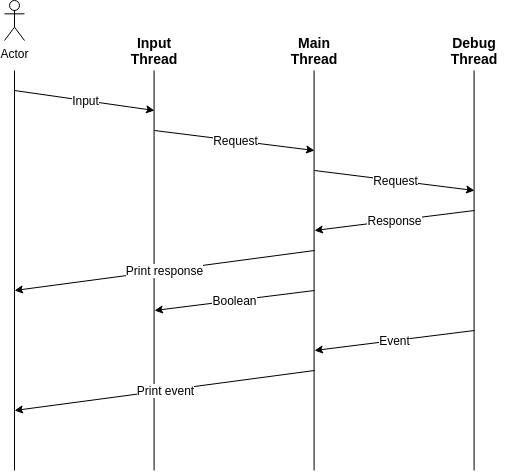
\includegraphics[width=0.9\textwidth]{cli_flow.png}
	\caption{A diagram showing the communication between the user/actor and the three different threads.}
	\label{fig:cliflow}
\end{figure}

